\section{Wie benutzt man diese Vorlage}
\subsection{Konfiguration und Generelles}
Diese Vorlage ist so aufgebaut, dass du nichts mehr konfigurieren oder einstellen musst.
Stattdessen kannst du dich auf das Schreiben deiner Arbeit konzentrieren.
Im Hauptverzeichnis liegt die Datei \verb|01_config.tex|.
In dieser Datei werden die Grunddaten deiner Arbeit festgelegt.
Dazu zählt auch die Sprache.
Hier kannst du entscheiden, ob du deine Arbeit auf Deutsch oder Englisch verfassen möchtest.
Je nachdem welche Sprache du verwendest, werden alle Inhalte automatisch in der entsprechenden Sprache dargestellt (außer natürlich dein geschriebener Text).
Außerdem legst du in dieser Datei dein Name, Titel, Prüfer und alles weitere fest.
Dies dient dazu, damit diese an entsprechender Stelle automatisch geladen werden können.
Möchtest du also zum Beispiel in deiner Danksagung den Erstprüfer erwähnen, so musst du nur den Befehl \verb|\reviewer| benutzen.

Außerdem empfehle ich, deinen Text sinnvoll in Dateien zu gliedern.
Du kannst zum Beispiel jedes Kapitel in eine Datei packen.
Ein Beispiel ist hier schon gegeben.
Über die Datei \verb|main.tex| werden dann deine Dateien eingebunden (siehe Zeile 154).
Um die Compile-Zeit zu steigern, kannst du auch nur einzelne Dateien laden.
Dies passiert in Zeile 12 in \verb|main.tex|.
Hier gibst du die Dateien an, an welchen du aktuell arbeitest.
Der Vorteil hierbei ist, dass Referenzen auf andere Kapitel oder Bilder aus anderen Kapitel dennoch dargestellt werden können, und keine Compile-Fehler auftreten.

Standardmäßig enthält die generierte PDF eine Coverseite.
Diese kannst du beim Drucken gut als erste Seite oder als Cover benutzen.
Brauchst du diese Seite nicht, kannst du Zeile 26 in \verb|main.tex| auskommentieren oder löschen.



\subsection{Nummerierung von Bilder, Tabellen etc.}
Bilder, Tabellen etc. werden automatisch nummeriert.
Was jedoch kurz für Verwirrung sorgen kann, ist die Art und Weise der Nummerierung.
Alle Elemente besitzen die erste Zahl entsprechend des Kapitels, in dem sie sich befinden.
Sprich, Abbildung 3.5 befindet sich in Kapitel 3.
Die zweite Zahl wird beginnend bei 1 und fortlaufend generiert.
Diese Art der Nummerierung wird häufig bei Abschlussarbeiten verwendet.



\subsection{Overleaf oder andere IDEA?}
Generell empfehle ich dir, jeden Satz in einer neuen Zeile im Editor zu beginnen.
Dies erleichert die Lesbarkeit deines Codes und ermöglicht, falls du mit der Overleaf Review Funktion arbeitest oder mit Git, bessere Kommentare durch deinen Betreuer.
Aufgrund der doch langen Compile-Zeit von Overleaf bei größeren Arbeiten empfehle ich die Verwendung von TexLive und Visual Studio Code für Windows (\href{https://blog.jakelee.co.uk/getting-latex-working-in-vscode-on-windows/}{Hier eine Anleitung}).
Über Git kannst du deine Arbeit sichern und dein Betreuer kann z.B. über Issues Anmerkungen machen.
Wenn du mit Visual Studio Code arbeitest und deine Sätze sehr lang sind, kannst du horizontales Scrollen vermeiden über \verb|View| $\rightarrow$ \verb|Word Wrap|



\subsection{Abkürzungen verwenden}
In der Datei \verb|02_abbreviations.tex| musst du deine Abkürzungen festlegen.
Einige Beispiele sind bereis in der Datei enthalten.
Möchtest du eine Abkürzung verwenden, benutze einfach den Befehl \verb|\ac{...}|.
Um die Plural-Form zu verwenden, benutze den Befehl \verb|\acp{...}|.
LaTeX erkennt automatisch, wenn du die Abkürzung das erste Mal verwendest und schreibt diese aus.
Außerdem werden im Abkürzungsverzeichnis nur die Abkürzungen dargestellt, die du auch verwendest.
Es ist also nicht schlimm, eine zu lange \verb|02_abbreviations.tex|-Datei zu haben.
Das Abkürzungsverzeichnis ist außerdem bereits automatisch alphabetisch sortiert.
Ansonsten passiert alles automatisch - außer die beiden Befehle benutzen brauchst du nichts weiter tun.
So sieht dann eine verwendete Abkürzung aus: \ac{API}



\subsection{Quellenangaben verwenden}
In der Datei \verb|references.bib| werden deine Quelle festgelegt.
Auch hier sind einige Beispiele bereits in der Datei vorhanden.
Um eine Quelle in deinem Text zu benutzen, verwende den Befehl \verb|\cite{...}|.
Wie bereits bei den Abkürzungen werden alle verwendeten Quellen automatisch in das Literaturverzeichnis geladen.
Eine verwendete Quellenangabe sieht dann am Ende so aus im Text \cite{test}.
Wenn du möchtest, kannst du den Zitier-Style ändern.
Dies geschieht über Zeile 52 und 53 in der Datei \verb|settings.sty|.
Jedoch empfehle ich für Abschlussarbeiten an der Fakultät IT die bereits hinterlegte numerische Zitierweise.

Zum organisieren deiner Quellen kann ich dir Zotero empfehlen.
Hier kannst du deine ganzen Quellen verwalten, sortieren, mit Tags versehen wie zum Beispiel "noch nicht gelesen", und vieles mehr.
Der Vorteil ist, dass du in Zotero die \verb|.bib|-Datei generieren lassen kannst und diese dann ganz einfach in deiner Thesis verwenden kannst.
Außerdem bietet Chrome eine Zotero-Erweiterung an.
Mit dieser können Paper, Artikel, Websiten etc. super schnell und unkompliziert als Quelle gespeichert werden, meist automatisch mit den richtigen Angaben wie Autoren, Datum, etc.
Außerdem werden in Zotero die PDFs gespeichert, heißt du musst beim nachlesen von Sachen in deinen Quellen nicht immer erst die PDF wieder im Netz suchen.



\subsection{Bilder einbinden}
Für Bilder ist bereits der Ordner \verb|/images| hinterlegt.
Speichere also alle Bilder dort.
Wenn möglich, vor allem bei Grafiken, sollte das PDF Format bevorzugt werden.
Dies ermöglicht eine scharfe Darstellung.
Um eigene Grafiken zu erstellen, empfehle ich dir \href{https://app.diagrams.net/}{app.diagrams.net/}.
Hier kannst du einfach und unkompliziert alles als PDF exportieren.
Falls du eine Grafik aus einer Quelle benutzt, empfehle ich dir, diese "nachzubauen" und anschließend einen Vermerk anzugeben mit Referent zum Original.

Das \verb|[b]| beschreibt, wie dein Bild floaten soll.
Generell wird empfohlen, auch bei den meisten Papern, dass Bilder entweder auf Seiten oben oder unten floaten sollen.
\verb|b| steht dabei für "bottom", also das Seitenende.
\verb|t| wird benutzt, um das Bild oben floaten zu lassen.
\verb|h| kannst du benutzen, um das Bild an genau dieser Stelle zu generieren.
Dies kann auch verwendet werden, falls es dein Erstprüfer erlaubt.
Generell gelten diese Floating-Optionen auch für Tabellen, Quellcode oder Pseudocode.

Zum Einbinden von Bildern, benutze den folgenden Code:
\begin{verbatim}
    \begin{figure}[b]
        \centering
        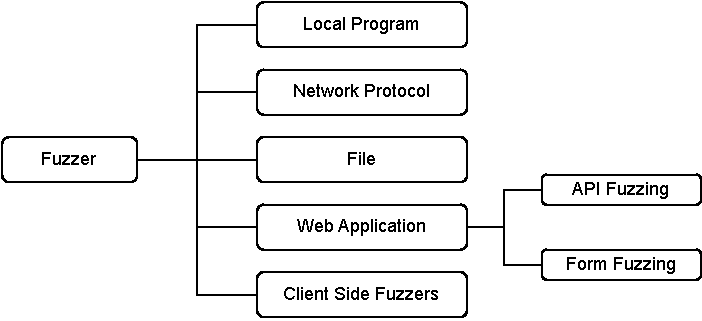
\includegraphics[width=0.85\textwidth]{example.pdf}
        \caption[Some Caption]{Some Caption (based on \cite{test})}
        \label{img:bla}
    \end{figure}
\end{verbatim}\noindent
Über \verb|width=0.85\textwidth| gibst du an, wie breit dein Bild sein soll.
Ich empfehle hier, einen Wert von 0.95 nicht zu überschreiten.

Über \verb|\caption| gibst du die Bildunterschrift an.
Falls du, wie zuvor erwähnt, auf eine Quelle verweisen möchtest, benutze die geschweiften Klammern.
Dies sorgt dafür, dass die Caption in den eckigen Klammern im Abbildungsverzeichnis dargestellt wird und die Caption in den geschweiften Klammern unter dem Bild selber.

Um auf das Bild verweisen zu können (wird in \autoref{sec:ref} erklärt), musst du den Befehl \verb|\label| benutzen und das Label definieren.
Dies wird anschließend benutzt, um das Bild zu refenzieren.
Hier kannst du dir ein Schema überlegen, zum Beispiel für Bilder "img:...".

Hier ist ein Beispiel, wie ein Bild mit der Floating-Option \verb|h| aussieht:
\begin{figure}[h]
    \centering
    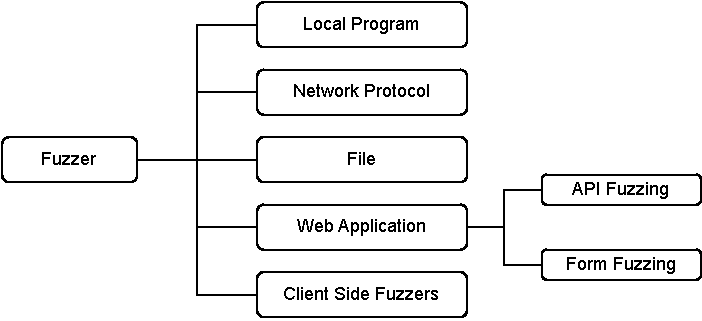
\includegraphics[width=0.75\textwidth]{example.pdf}
    \caption[Some Caption]{Some Caption (based on \cite{test})}
    \label{img:bla}
\end{figure}



\subsection{Tabellen einbinden}
Das Einbinden von Tabellen funktioniert prinzipiell genau gleich wie mit Bilder.
Es gibt die Floatin-Option, eine Caption sowie ein Label.
Auch hier kannst du optional für die Caption eckige Klammern benutzen.
Hier ist ein Beispiel für eine Tabelle.
Schaue dir einfach den Code an, dieser ist selbsterklärend.
\begin{table}[h]
    \centering
    \begin{tblr}{
            width = \linewidth,
            hlines,
            vlines,
        }
        \textbf{Fuzzer} & \textbf{Test 2}     \\
        APIFuzzer       & \color{red}failed   \\
        OFFAT           & \color{red}failed   \\
        openapi-fuzzer  & \color{red}failed   \\
        RESTler         & \color{red}failed   \\
        RestTestGen     & \color{green}passed \\
    \end{tblr}
    \caption{Some Caption}
    \label{tbl:bla}
\end{table}\noindent



\subsection{Quellcode einbinden}
Für das Einbinden von Quellcode wird das Verzeichnis \verb|\code| benutzt.
Hier legst du einfach deine Quellcodedatien ab, welche du darstellen möchhtest.
Quellcode bindest du über den folgenden Befehl ein:
\begin{verbatim}
    \lstinputlisting[float=b, caption=Some Caption, label=lst:bla]{redos.ts}
\end{verbatim}\noindent
Auch hier können die bereits beschriebenen Float-Optionen verwendet werden.
Aus Gründen der Übersichtlichkeit verzichtet meine Vorlage auf farbliches Hervorheben im Quellcode.
Generell solltest du nur die relevanten Zeilen im Quellcode darstellen, welche absolut relevant sind.
Die vollständige Datei kannst du dann zum Beispiel im Anhang einfügen.
Benutze hierfür die beispielhafte Datei \verb|/content/99_appendix.tex|
\lstinputlisting[float=h, caption=Some Caption, label=lst:bla]{redos.ts}



\subsection{Pseudocode einbinden}
Es kann vorkommen, dass du Pseudocode oder Algorithmen zum Beispiel im Rahmen eines Designs einbinden möchtest.
Hier siehst du ein Beispiel, wie ein Algorithmus eingebunden ist.
Schaue dir einfach den Code dazu an, dieser ist selbsterklärend.
Auch hier gibt es wieder die bekannten Elemente wie die Floating-Option, die Caption und das Label.
\begin{algorithm}[h]
    \caption{Handling basic authentication via configuration file}
    \label{pseudo:bla}
    \begin{algorithmic}[1]
        \Function{GetAuthData}{config}
        \State...
        \State \Return userID, password
        \EndFunction

        \Function{GenerateBasicAuthHeader}{userID, password}
        \State credentials $\leftarrow$ userID + `:' + password
        \State encodedCredentials $\leftarrow$ \Call{Base64Encode}{credentials}
        \State authHeader $\leftarrow$ `Authorization: Basic ' + encodedCredentials
        \State \Return authHeader
        \EndFunction

        \vspace{3pt}
        \State configFilePath $\leftarrow$ `path/to/config/file'
        \State userID, password $\leftarrow$ \Call{GetAuthData}{configFilePath}
        \State authHeader $\leftarrow$ \Call{GenerateBasicAuthHeader}{userID, password}
        \State ...
    \end{algorithmic}
\end{algorithm}


\subsection{Referenz zu Kapiteln, Bildern, Tabellen etc.}
\label{sec:ref}
Du solltest darauf achten, dass jedes Bild, jede Tabelle, jeder Quellcode etc. auch im Text erwähnt wird.
Dabei kannst du mit Hilfe des \verb|\autoref{...}| Befehls schnell und unkompliziert auf das Element verweisen.
Innerhalb der geschweiften Klammern schreibst du das Label, das du definiert hast.
Alle refenzierten Inhalte sind außerdem anklickbar.
Hier ein Beispiel:

Zu diesem Zweck fügen wir einen neuen Pfad \texttt{redos} hinzu, der mit der HTTP-Methode \texttt{GET} aufgerufen wird, wie in \autoref{lst:bla} dargestellt.



\subsection{ToDos}
In diese Vorlage ist die Verwendung von ToDos integriert.
Dies kann dir dabei helfen, deinen aktuellen Fortschritt besser zu verfolgen oder auch eine bessere Kommunikation mit deinem Betreuer ermöglichen.
Die folgenden ToDos stehen dabei zur Verfügung:
\begin{verbatim}
    \toDo{XY muss noch eingebaut werden}
    \improvement{Du könntest noch etwas genauer über AB schreiben}
    \approve
    \approved
\end{verbatim}\noindent
\toDo{XY muss noch eingebaut werden}
\improvement{Du könntest noch etwas genauer über AB schreiben}
\approve
\approved
Falls du dieses Feature nicht brauchst, kommentiere Zeile 26 in \verb|01_config.tex| ein und lösche Zeile 27.
Wenn du die ToDos verwendest und am Ende deine finale PDF generieren möchtest, brauchst du nicht alle ToDos manuell entfernen. Hierzu kannst du auch einfach Zeile 26 in \verb|01_config.tex| einkommentieren und Zeile 27 löschen.